%Reporte sobre la actividad del producto 6
\documentclass[notitlepage,12pt]{article}

%El documento estara en español, usar paquete en español
\usepackage[spanish]{babel}
\selectlanguage{spanish}
\usepackage[utf8]{inputenc}
%Permite colores
%Permite incorporar imagenes
\usepackage{graphicx}
\usepackage{color}
%Escribir formulas matematicas
\usepackage{amsmath}
%topmatter (titulo, autor, fecha)
\title{Movimiento de proyectiles incluyendo fricci\'on del aire}
\author{Hugo de Jes\'us Valenzuela Chaparro}
\date{\today}

\begin{document}
\maketitle

\section{Tiro parab\'olico con fricci\'on del aire}
El estudio de la trayectoria de un proyectil es un problema que ha sido de inter\'es por mucho tiempo. Sea 
con aplicaciones militares o en los deportes. Para estudiarse se separa en dos tipos de movimientos, un
movimiento rectil\'ineo uniforme con velocidad constante en el eje x y un movimiento rectil\'ineo uniformemente
acelerado en el eje y (con la aceleraci\'on de la gravedad). Las ecuaciones de movimiento del proyectil sin considerar
la fricción están dadas por las ecuaciones:
$x=vtcos\theta$
$y=vtsin\theta-\frac{1}{2}gt^2$
donde x y y son las variables de posición del proyectil, v es la rapidez inicial con la que se lanzó, g la aceleración 
debida a la gravedad y $\theta$ el \'angulo de lanzamiento inicial. Para determinar de forma unívoca la trayectoria de un proyectil, 
solo es necesario conocer 2 cantidades: la rapidez inicial v y el ángulo $\theta$  con el que se lanzó.

Todo objeto de masa $m$ que se mueve a muy alta velocidad en un fluido de densidad $\rho$ ,  experimenta una fuerza de arrastre $F_r$ 
contraria a la dirección de su movimiento y es  dada por la ecuación $F_r=\frac{1}{2}\rho v^2C_DA$. Donde $v$ es la magnitud del vector 
velocidad del objeto, $C_D$ es  el coeficiente de arraste (adimensional), $A$ es el área transversal presentada por el objeto. 
Por ejemplo, para una esfera el área transversal es $A=\pi r^2$ , y  el coeficiente de arrastre es $C_D=0.47$.
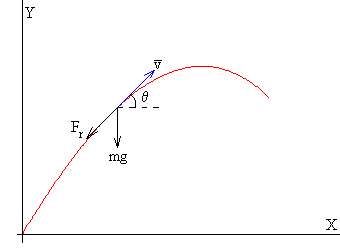
\includegraphics{parabolicfriction}


\section{C\'odigo en Fortran}
A continuaci\'on se presenta el c\'odigo de un programa en Fortran que calcula la trayectoria de un proyectil considerando la friccion
del aire y tambi\'en no consider\'andola.

\begin{verbatim}
!constantes
MODULE constantes
 IMPLICIT NONE
 real, parameter :: pi = 4.0*atan(1.0), g=9.81, den=1.19 
 INTEGER, PARAMETER :: npts=5000
!Coeficiente de arrastre de la esfera
REAL,PARAMETER :: dc=0.47
END MODULE constantes
!Subrutina para trayectoria sin friccion
SUBROUTINE SinFriccion(x0,y0,u,a_grados,mx,my,ft)
  
      
       USE constantes
       implicit none  
       !Defining constants:  
      
       real :: u, a, t, a_grados, my, mx, ft, Vx, Vy, FA,x0,y0  
       
       real:: x(150),y(150)  
          integer :: i 

       !where g is gravity, pi is "pi"   
       !u is object's initial velocity   
       !a is object's initial angle (grades)
       !t is time during the simulation   
       !x and y are arrays with 150 rows   
       !Seek user input   
       !write(*,*) 'Ingresa el angulo de lanzamiento (Real)'   
       !read *, a_grados   
       !write(*,*) 'Ingresa la velocidad inical del proyectil en m/s (Real)'   
       !read *, u   
       !Convertir angulo a radianes  
       a = (a_grados*pi)/180.0   
       !Calcular componentes de la velocidad en x (Vx) e y (Vy)
       IF (a_grados == 90.0) THEN
       Vx=0.0
       Vy=u
       ELSE IF (a_grados == 0.0) THEN
       Vx=0.0
       Vy=0.0
       ELSE
       Vx=u*cos(a)
       Vy=u*sin(a)
       END IF
        
   !Calcular el tiempo que el objeto esta en el aire, siendo el mismo
   !en las componentes x e y
   ft=(2.0*Vy)/g
 
  
   !calcular altura maxima
   my=(Vy**2)/19.62
   
   !Print results 
  ! print*, "Velocidad inicial:", u,"m/s"
   !print*, "Angulo de lanzamiento (grados):", a_grados
  ! print*, "Tiempo total de vuelo:", ft, "s"
  ! print*, "La altura maxima es:", my,"m"
   
    
       !open .dat file and start writing on it using the algorithm   
       open(1, file='sinfriccion.dat')   
         
       
       do i=1,npts 
           
            !displacement of object in x and y direction   
            t = (float(i)*0.1)   
            x(i) = x0+ Vx*t   
            y(i) = y0+ (Vy*t)-(4.905*t*t)   
            !write output in file "proj.dat" for plotting   
            write(1,1001) x(i), y(i)   
            1001 format (f11.5, f11.5)
            !kill the loop when the object hits the ground   
            IF (y(i)<0) exit  
       end do 
       close(1)   
       !close file 

   
  !Desplazamiento en la direccion x hasta que el objeto toca el suelo
   mx=x(i)
   ! print*, "El desplazamiento total en la direccion x es:", mx,"m"
  



END SUBROUTINE SinFriccion
!Subrutina para trayectoria con friccion del aire
SUBROUTINE ConFriccion (x0,y0,v0,a_grados,mxf,myf,ftwf)
    USE constantes
    IMPLICIT NONE
REAL,DIMENSION (0:npts) :: xf, yf,vxf, vyf, ayf, axf, tf
REAL :: x0,y0,v0,a_grados,mxf,myf,ftwf
REAL :: masa,radio,a,Dom,mx,area
INTEGER :: i
a = (a_grados*pi)/180.0
PRINT*, "Escribe la masa de la esfera (kg)"
READ*, masa
PRINT*, "Escribe el radio de la esfera (m)"
READ*, radio
area=pi*radio*radio
!Condiciones iniciales
xf(0)=x0
yf(0)=y0
vxf(0)=v0*cos(a)
vyf(0)=v0*sin(a)
Dom=((area*den*dc)/2.0)/masa
axf(0)=-Dom*vxf(0)*vyf(0)
ayf(0)=-g-(Dom*vyf(0)*vyf(0))
tf(0)=0

 !open .dat file and start writing on it using the algorithm  

open(2, file='confriccion.dat')   
      write (2,1001) xf(0), yf(0)
      1001 format (f11.5, f11.5)
       
       do i=0,npts 
           
              
            tf(i+1)= tf(i)+0.01  
            vxf(i+1)=vxf(i)+axf(i)*tf(i+1)
            vyf(i+1)=vyf(i)+ayf(i)*tf(i+1)
            axf(i+1)=(-Dom)*vxf(i)*vxf(i)
            ayf(i+1)=-g-(Dom*vyf(i)*vyf(i))
            xf(i+1)=xf(i)+vxf(i)*tf(i+1)+((axf(i)*tf(i+1)*tf(i+1))/2.0)
            yf(i+1)=yf(i)+vyf(i)*tf(i+1)+((ayf(i)*tf(i+1)*tf(i+1))/2.0)  
            !write output in file "proj.dat" for plotting   
            write(2,1001) xf(i+1), yf(i+1)   
            !write (2,1001) x(i), y(i)
            !1001 format (f11.5, f11.5)
            !kill the loop when the object hits the ground   
            IF (yf(i)<0) exit  
       end do 
       close(2)   
       !close file 

!Resultados
ftwf=tf(i)*10.0
myf=maxval(yf)
mxf=xf(i)

END SUBROUTINE ConFriccion

!Programa maestro
PROGRAM ProyectilesFriccion
        USE constantes
        IMPLICIT NONE
        REAL :: v0,a_grados,mx,my,ft,x0,y0,mxf,myf,ftwf,Et,Ex,Ey
        REAL,DIMENSION (0:npts) :: x, y,vx, vy, ay, ax, t
PRINT*, "Este programa calcula el alcance en x y y en un tiro parabolico, &
& para cuando hay friccion y cuando no la hay"
PRINT*, "Ingresa la posicion inicial x0 y y0 (m), luego el angulo inicial (grados) y &
& la velocidad inicial (m/s), respectivamente"
READ*,x0,y0,a_grados,v0

!Llamar subrutinas
CALL SinFriccion(x0,y0,v0,a_grados,mx,my,ft)
CALL ConFriccion(x0,y0,v0,a_grados,mxf,myf,ftwf)

Et=((ABS(ftwf-ft))/ftwf)*100.0
Ex=((ABS(mxf-mx))/mxf)*100.0
Ey=((ABS(myf-my))/myf)*100.0

PRINT*, "Sin friccion, los resultados son:"
PRINT*, "El desplazamiento total en x es",mx, "m"
PRINT*, "La altura maxima es", my, "m"
PRINT*, "El tiempo total de vuelo es" ,ft, "s"
PRINT*, "-------------------------------------------------------"
PRINT*, "Con friccion, los resultados son:"
PRINT*, "El desplazamiento total en x es", mxf, "m"
PRINT*, "La altura maxima es", myf, "m"
PRINT*, "el tiempo total de vuelo es", ftwf, "s"
PRINT*, "-------------------------------------------------------"
PRINT*, "Error relativo poncertual al no considerar la friccion del aire:"
PRINT*, "En el desplazamiento x es del",Ex,"%"
PRINT*, "En el desplazamiento y es del",Ey,"%"
PRINT*, "En el tiempo total de vuelo es del",Et,"%"
END PROGRAM ProyectilesFriccion
\end{verbatim}

\section{Resultados del programa corriendo}
\subsection{$\theta=30$}
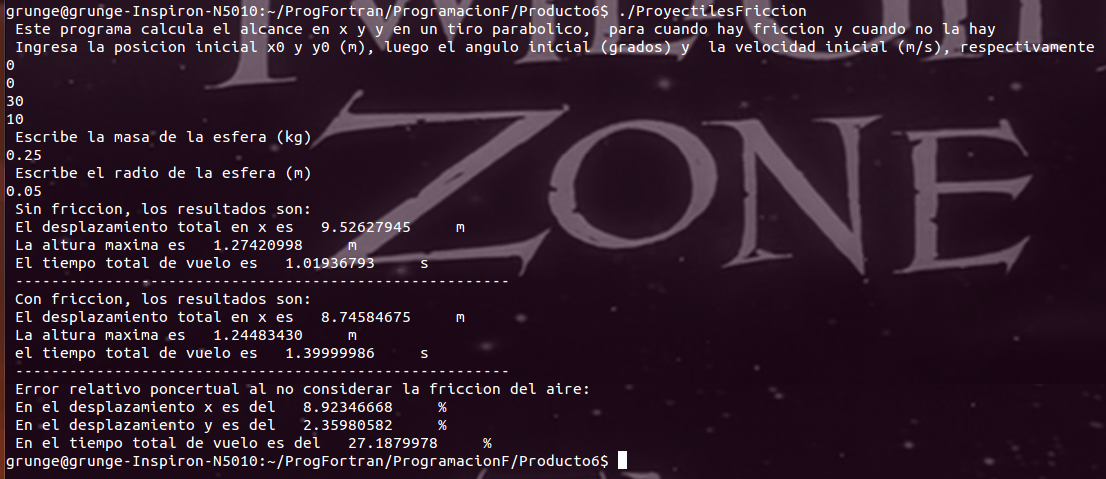
\includegraphics[scale=0.4]{theta_30}


Sin fricci\'on

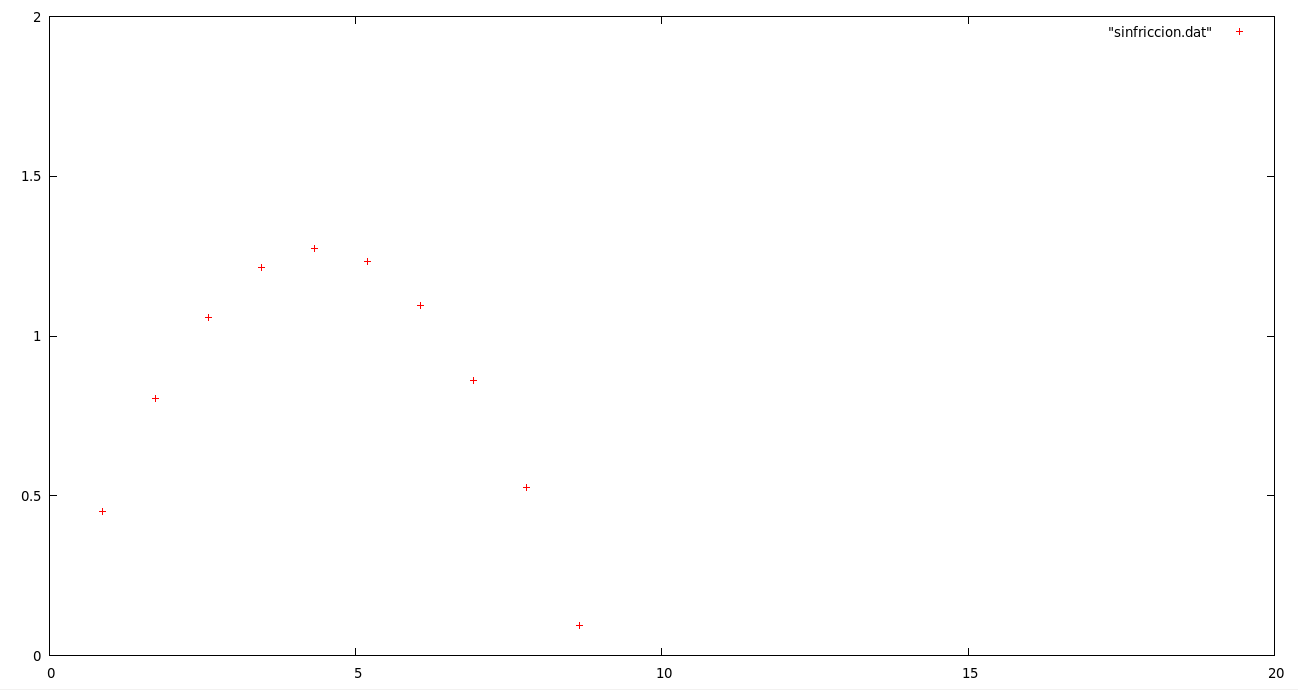
\includegraphics[scale=0.3]{theta_30_plot_nofriction}

Con fricci\'on

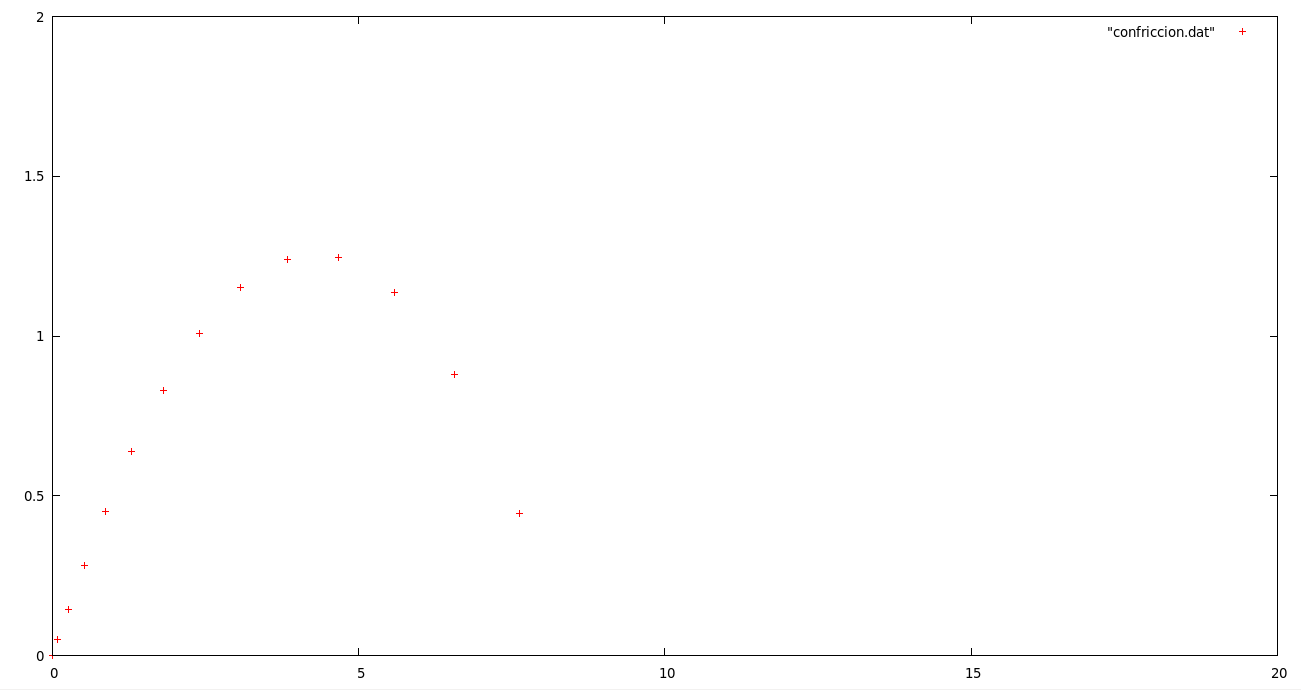
\includegraphics[scale=0.3]{theta_30_plot_friction}

\subsection{$\theta=60$}
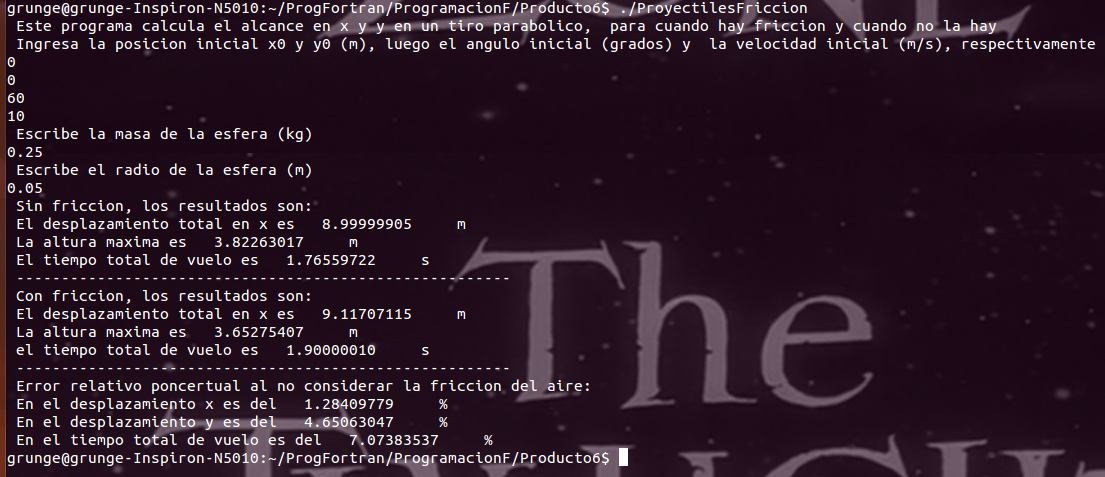
\includegraphics[scale=0.4]{theta_60}


Sin fricci\'on

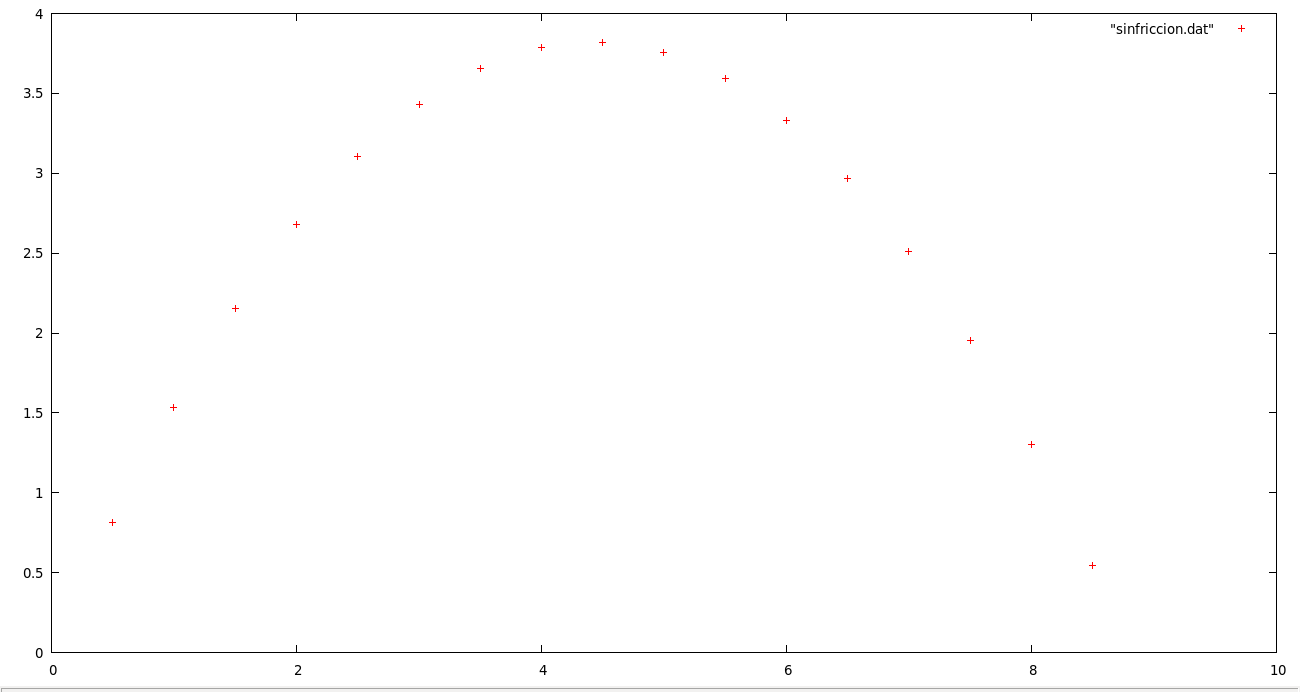
\includegraphics[scale=0.3]{theta_60_plot_nofriction}

Con fricci\'on

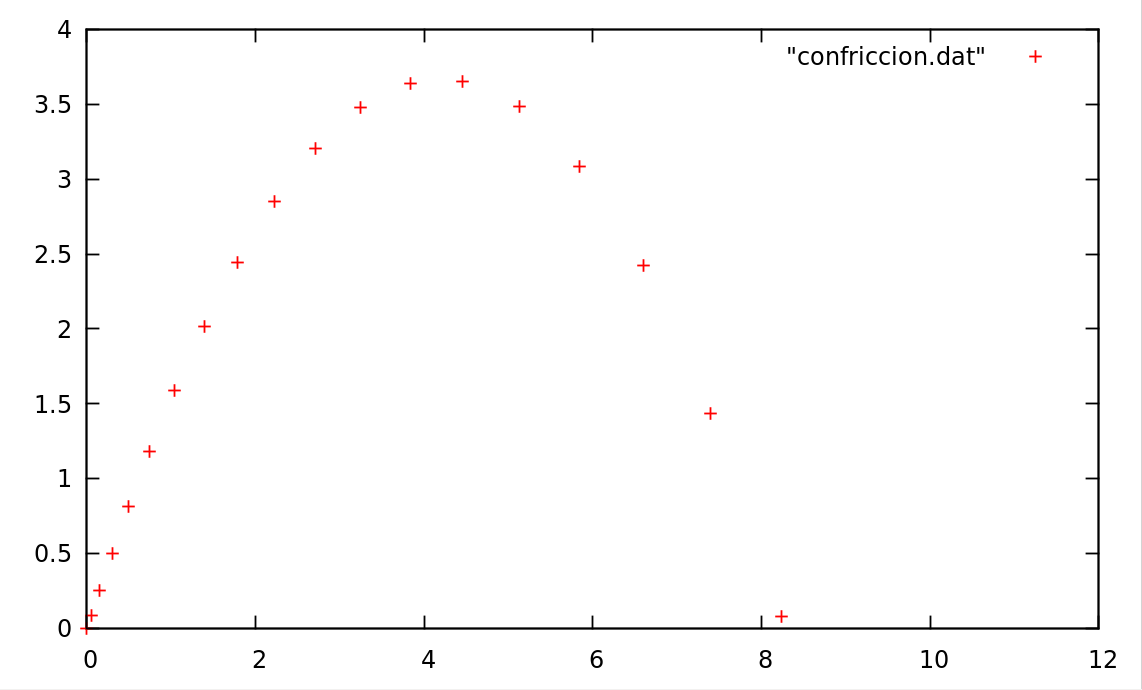
\includegraphics[scale=0.3]{theta_60_plot_friction}

\subsection{$\theta=45$}
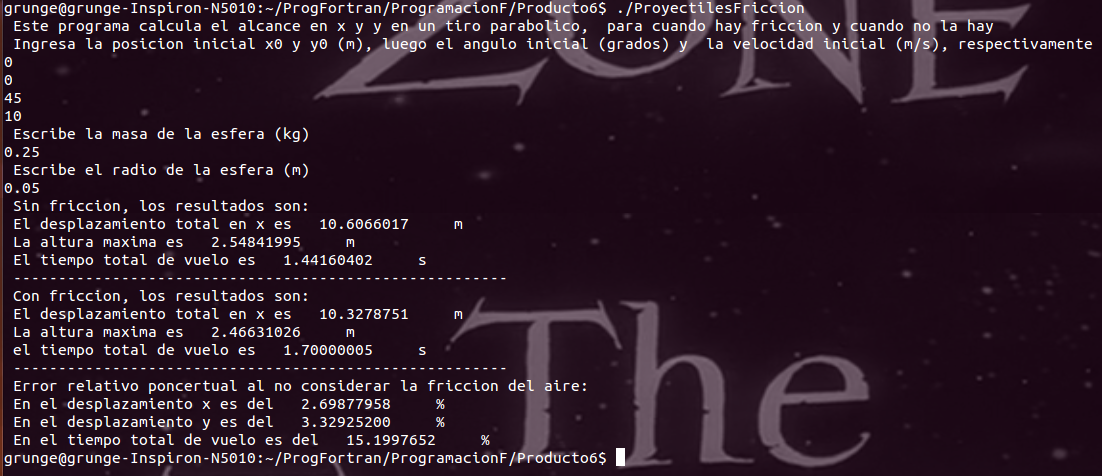
\includegraphics[scale=0.4]{theta_45}


Sin fricci\'on

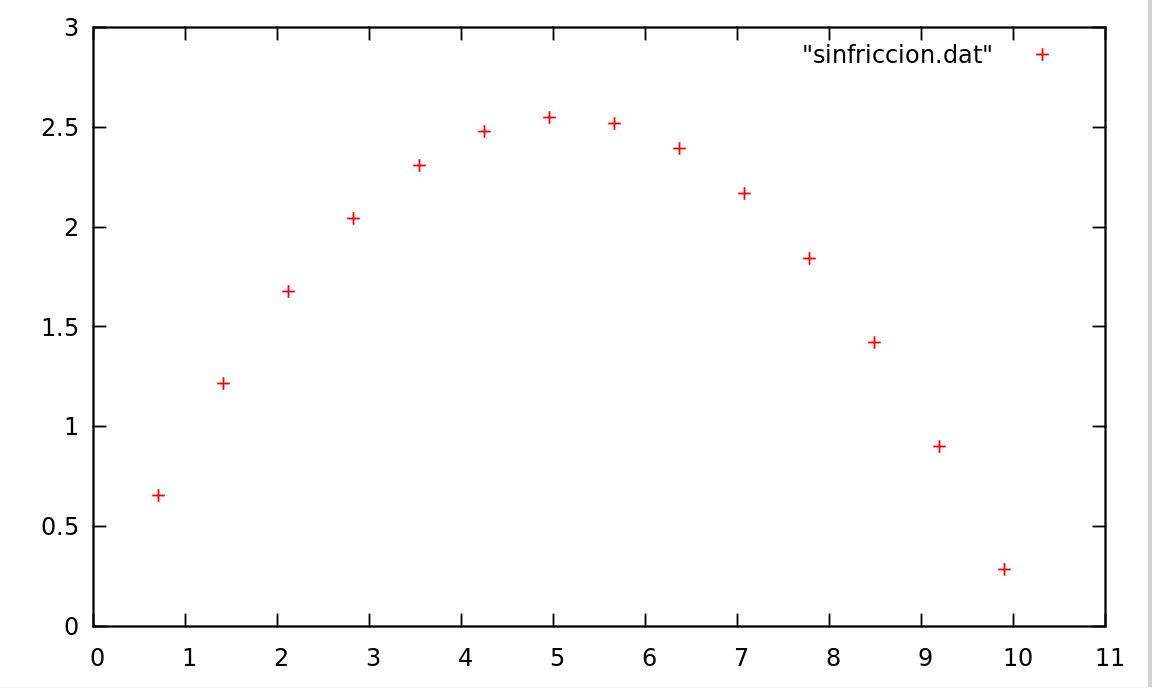
\includegraphics[scale=0.3]{theta_45_plot_nofriction}

Con fricci\'on

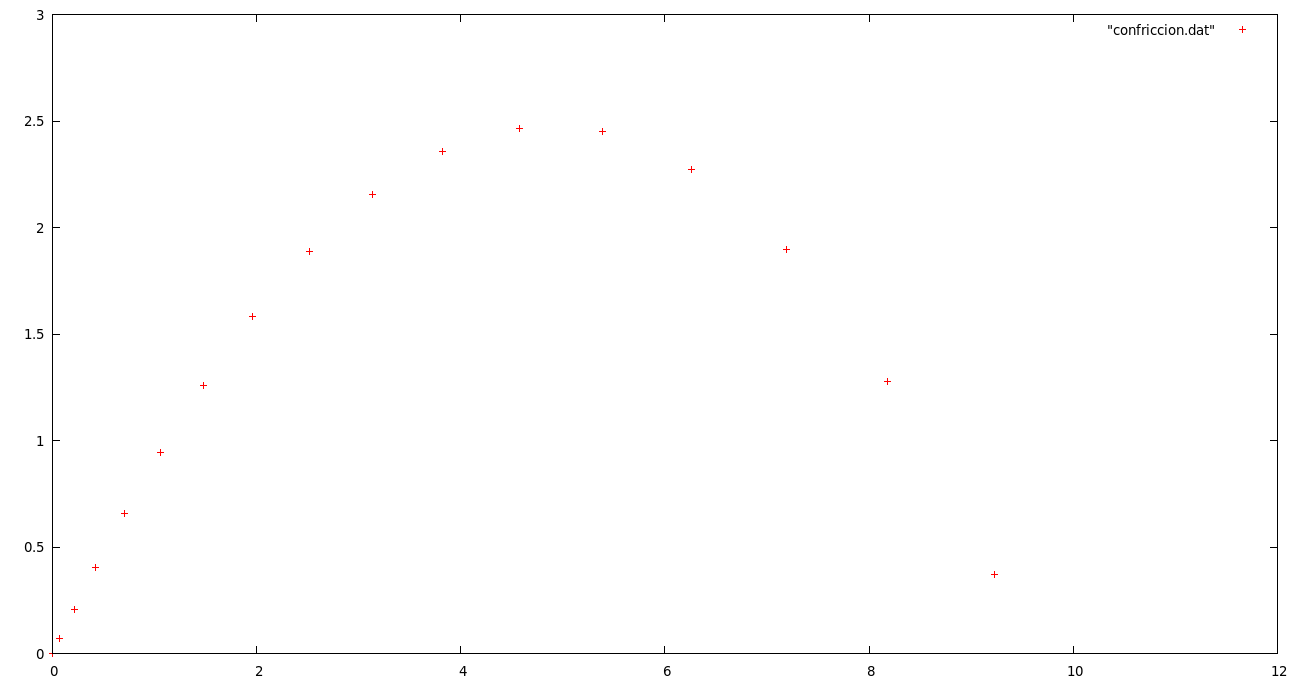
\includegraphics[scale=0.3]{theta_45_plot_friction}



Los resultados tiene sentido, pues cuando hay fricci\'on se puede apreciar que las distancias m\'aximas en x e y son menores
que cuando no la hay. Adem\'as el tiempo total de vuelo es mayor cuando hay fricci\'on, y en el programa corriendo puede verse,
esto se debe a que cuando el objeto va cayendo el aire act\'ua como ``paraca\'idas'' debido a la fricci\'on generada.



\end{document}
